\chapter{METODOLOGIA}

\section{Modelagem dinâmica de uma impressora 3D}
Para a modelagem do sistema mecânico são consideradas as seguintes simplificações:
\begin{itemize}
    \item Não existe escorregamento nem perda de potência na interação entre a polia e a correia
    \item A correia apresenta um comportamento equivalente à uma mola e um amortecedor em paralelo
    \item O bico injetor é um corpo rígido uniforme de geometria simples
\end{itemize}

Para a modelagem dinâmica dos eixos X e Y da impressora 3D, 
é considerado que os eixos são completamente independentes, 
a flexibilidade da correia é aproximada utilizando um conjunto 
mola amortecedor e a transmissão de movimento e torque dos 
motores é considerada como ideal e não será abordada.
Assim duas posições de estudo surgem para cada eixo, uma delas 
representa a posição ideal, caso o sistema não possuiesse nenhuma flexibilidade
ou perda, que também é a posição desejada pelo usuário ($x_b$). 
A segunda posição considera as forças inerciais e a 
flexibilidade introduzida pela correia, ou seja, a posição real simulada pelo modelo
e no caso empírico a posição real ($x$) como na figura \ref{fig:din_model}.

\begin{multline}
    \label{eq:mov_impressora}
    \\
    m \ddot{x_p} + c(\dot{x_p} - \dot{x_b}) + k(x_p-x_b) = 0 \\
    - \frac{c}{m}(\dot{x_p} - \dot{x_b}) - \frac{k}{m}(x_p-x_b) = \ddot{x_p} \\
    - \frac{c}{m} \dot{x_p} - \frac{k}{m} x_p + \frac{c}{m} \dot{x_b} + \frac{k}{m} x_b  = \ddot{x_p} \\
\end{multline}

\subsection{Espaço de estados}
A formulação de espaço de estados foi utilizada com intuito de facilitar as operações e
a a solução do sistema, dado sua característica de dividir uma equação diferencial
de ordem superior em um sistema de equações diferenciais de ordem 1 com um número maior de equações.
O modelo dinâmico do sistema é apresentado na formulação de espaço de estados 
na equação \ref{eq:simp_state_space_din_model}, onde $\dot x$ $x$ $A$ $u$ $B$.
Baseado na equação \ref{eq:mov_impressora} expandimos as matrizes e vetores na equação 
\ref{eq:espaco_de_estados_din_model}.
Como o modelo dos eixos x e y estão sendo considerados como iguais, também podemos utilizar a equação 
\ref{eq:espaco_de_estados_din_model} para a base do eixo y.

\begin{equation}
    \label{eq:simp_state_space_din_model}
    \dot x = A*x+B*u
\end{equation}

\begin{equation}
    \label{eq:espaco_de_estados_din_model}
    \begin{bmatrix}
        \dot{x_p} \\
        \ddot{x_p} \\
        \dot{y_p} \\
        \ddot{y_p}
    \end{bmatrix}
    =
    \begin{bmatrix}
        0 & 1 & 0 & 0 \\
        -\frac{k_x}{m_x} & -\frac{c_x}{m_x} & 0 & 0 \\
        0 & 0 & 0 & 1 \\
        0 & 0 & -\frac{k_x}{m_x} & -\frac{c_x}{m_x}
    \end{bmatrix}
    \begin{bmatrix}
        x_p \\
        \dot{x_p} \\        
        y_p \\
        \dot{y_p} \\
    \end{bmatrix}
    +
    \begin{bmatrix}
        0 & 0 & 0 & 0 \\
        \frac{k_x}{m_x} & \frac{c_x}{m_x} & 0 & 0 \\
        0 & 0 & 0 & 0 \\
        0 & 0 & \frac{k_x}{m_x} & \frac{c_x}{m_x}
    \end{bmatrix}
    \begin{bmatrix}
        x_b \\
        \dot{x_b}  \\
        y_b \\
        \dot{y_b} 
    \end{bmatrix}
\end{equation}

\section{Geração de Comando}

A geração de comando se inicia na leitura do Gcode para a obtenção dos movimentos e velocidades desejadas.
Foi considerado no mapeamento do Gcode apenas comandos G1, extraindo
as informações dos eixos X, Y e do \textit{feedrate} (F). Com base nesses valores
uma matriz 3 por n é criada, n sendo o número de comandos lidos do arquivo Gcode.
Em geral a unidade de F em arquivos Gcode gerados pelos fatiadores se dão em milímetros por minuto,
mas é convertida para milímetros por segundo na construção da matriz de entrada.

\subsection{Curva trapezoidal de velocidade}

A partir da matriz de entrada e das velocidades finais e iniciais dos movimentos estabelecido pelos comandos do Gcode,
utilizamos a função responsável por gerar a curva trapezoidal de velocidades.

Essa função constroi a curva de velocidade trapezoidal a partir dos dados
de entrada, sendo estes o deslocamento do movimento, as velocidades iniciais, velocidades finais e a velocidade desejada.
Para identificar se a velocidade desejada será alcançada é calculado a velocidade pico ($v_p$)
que é obtida extrapolando retas com as inclinações da aceleração na velocidade incial e final.
É possível obter a velocidade de pico através da equação \ref{eq:v_p}.

\begin{figure}[!htb]
    \centering
    \caption{Curva de velocidade trapezoidal}
    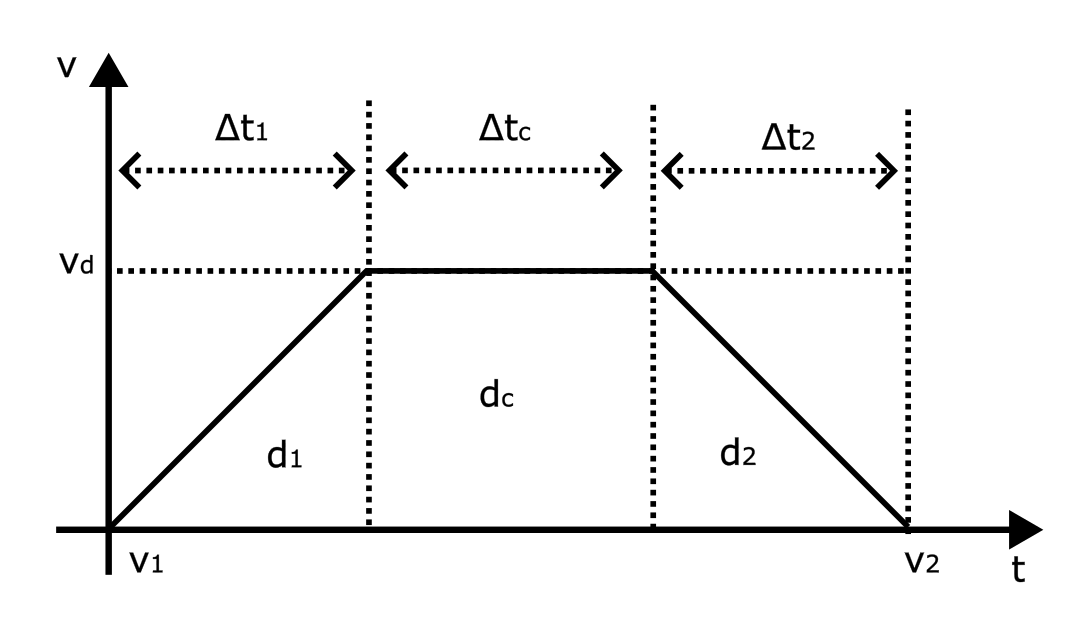
\includegraphics[scale=0.4]{trap_curv}

    \label{fig:trap_curv}
\end{figure}

\begin{figure}[!htb]
    \centering
    \caption{Curva de velocidade triangular}
    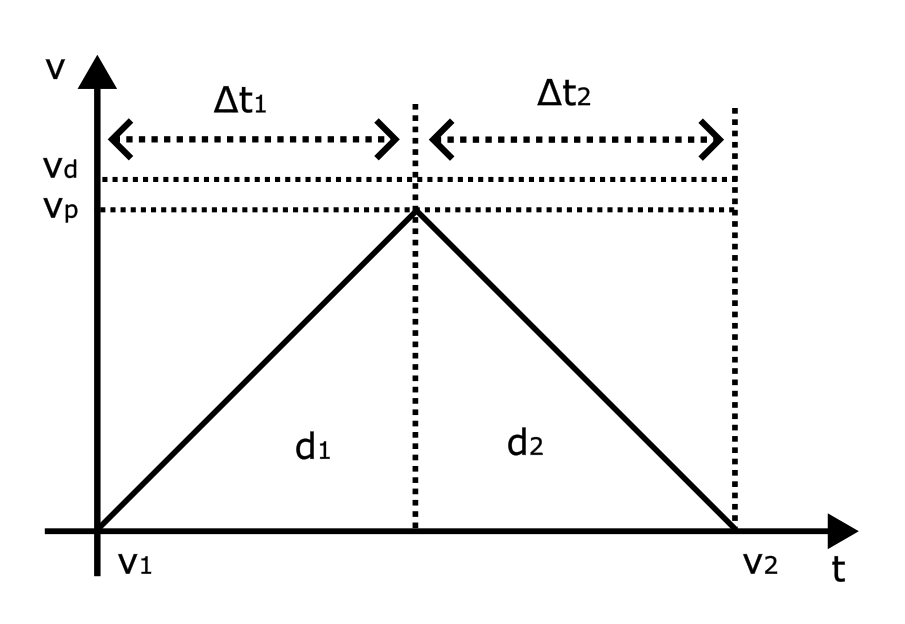
\includegraphics[scale=0.4]{triang_curv}

    \label{fig:triang_curv}
\end{figure}

\begin{equation}
    \label{eq:v_p}
    v_p = \sqrt{\frac{(v_1^2+v_2^2)}{2}+a*d}
\end{equation}

A partir da comparação da velocidade pico com a velocidade desejada, indicada pelo \textit{feedrate} disponibilizado no Gcode,
é possível determinar se a velocidade desejada será alcançada e assim determinar o perfil das curvas e como serão calculadas.
Caso a velocidade de pico for maior do que a velocidade desejada, temos 3 fases de deslocamento
que podem ser calculadas pelas equações \ref{eq:des_seg_a} e \ref{eq:des_seg_no_a}.
Caso a velocidade de pico seja igual ou menor do que a velocidade desejada, teremos 2 fases de deslocamento
que são calculadas a partir da equação \ref{eq:des_seg_a}.

\begin{equation}
    \label{eq:des_seg_a}
    d_1 = \frac{(v_d^2-v_1^2)}{(2*a)}
\end{equation}

\begin{equation}
    \label{eq:des_seg_a}
    d_2 = \frac{(v_2^2-v_d^2)}{(2*a)}
\end{equation}

\begin{equation}
    \label{eq:des_seg_a}
    d_1 = \frac{(v_p^2-v_1^2)}{(2*a)}
\end{equation}

\begin{equation}
    \label{eq:des_seg_a}
    d_2 = \frac{(v_2^2-v_p^2)}{(2*a)}
\end{equation}

\begin{equation}
    \label{eq:des_seg_no_a}
    d_c = d-(d_1+d_2)
\end{equation}

É possível calcular também os intervalos de tempo dessas fases, através das 
equações \ref{eq:dt_seg_a} e \ref{eq:dt_seg_no_a}.

\begin{equation}
    \label{eq:dt_seg_a}
    t_1 = \frac{(v_d-v_1)}{a}
\end{equation}

\begin{equation}
    \label{eq:dt_seg_a}
    t_2 = \frac{(v_2-v_d)}{a}
\end{equation}

\begin{equation}
    \label{eq:dt_seg_no_a}
    t_c = \frac{d_c}{v_d}
\end{equation}

\begin{equation}
    \label{eq:dt_seg_a}
    t_1 = \frac{(v_p-v_1)}{a}
\end{equation}

\begin{equation}
    \label{eq:dt_seg_a}
    t_2 = \frac{(v_2-v_p)}{a}
\end{equation}

% \begin{equation}
%     \label{eq:delta_vel}
%     \Delta v = v_f-v_i
% \end{equation}

Esses passos resultam em uma nova matriz contendo informações
sobre o a variação da posição, do tempo, da velocidade e sobre a aceleração e 
direção de deslocamento nos pontos iniciais e finais do Gcode e também nos pontos
onde existe uma alteração na aceleração.

\subsection{Interpolação}

A partir dos pontos de posição, velocidade, aceleração e tempo de cada eixo, é utilizada uma função de interpolação esses intervalos em pontos intermediarios
baseados em um passo de tempo definido para esta interpolação.
Para se dividir esses intervalos é possível utilizar a equação \ref{eq:N_steps}
calculando o número de passos neste intervalo, anexando à matriz os passos de tempo e por fim
o restante do intervalo, calculado pela equação \ref{eq:dt_interpol_last_step}.
Com base nestes passos de tempo, é possível calcular o deslocamento para cada um destes passos
através da equação \ref{eq:delta_des_interpol}.

\begin{equation}
    \label{eq:N_steps}
    N = \lceil\frac{\Delta t}{\Delta p}-1\rceil
\end{equation}

\begin{equation}
    \label{eq:dt_interpol_last_step}
    \Delta t_f= \Delta t - \Delta p*N 
\end{equation}

\begin{equation}
    \label{eq:delta_des_interpol}
    \Delta d_i = \Delta v_i*\Delta t_i+ \frac{a_s*\Delta t_i^2}{2} 
\end{equation}

A partir dos vetores de direção e da função acumuladora que se consite em acumular os valores de um vetor.
Obtemos uma matriz de posições, velocidades e tempo.

% \begin{equation}
%     \label{eq:acumulator_function}
%         s(k) = s(k)+s(k-1) 
% \end{equation}

\section{FMINCON}

\subsection{Configurações da função}
Foi utilizado o seguinte conjunto de configurações opcionais da função (tabela \ref{tab:fmincon_options}).
As configurações não indicadas se mantem na configuração padrão, que pode ser encontrada nos manuais da mesma.

\begin{table}
    \begin{center}
    \caption{Parâmetros opcionais da FMINCON}
    \label{tab:fmincon_options}
    \begin{tabular}{c c}
        Opção & Valor \\ \hline
        TolFun & 0.000000001 \\
        MaxIter & 100000 \\
        Display & iter \\
        DiffMinChange & 0.0001 \\
        Algorithm & interior-point \\
        StepTolerance & 1e-12 \\
        MaxFunEvals & 700000  \\ \hline
    \end{tabular}
    \end{center}
\end{table}

\subsection{Restrições lineares e limites de borda}
Não foi utilizado nenhuma restrição linear nessa otimização.
Os limites superiores (\textit{upperbound}) e inferiores (\textit{lowerbound}) foram definidos
baseados nos limites físicos da impressora (0 a 200 milímetros) para as posições $x_b$ e $y_b$.

\subsection{Restrições não lineares}
A função para as restrições não lineares foi implementada com base nas equaqções \ref{eq:state_center_segment},
\ref{eq:state_dot_center_segment}, \ref{eq:defect_calc}, \ref{eq:input_value_center_segment} de maneira a
popular a variável de restrições de igualdades com os valores do defeito dos segmentos ($\Delta$) e também
com os valores iniciais. 
Além disso, foi utilizado também como restrição de equalidade a arrancada, atrelado a um condicional para que
se comporte como uma inequalidade.
A variável de restrições de inequalidades não foi populada, os motivos são apresentados
na seção de resultados e discussão.

\subsection{Função objetivo}
Foram realizados alguns testes com funções objetivo e seus resultaods são apresentados na seção de resultados e discussão,
entretanto a função objetiva foi definida como zero, ou seja, pra qualquer valor ela retornara zero nas chamadas da FMINCON.

\section{Solução da trajetória da base}

É considerada como trajetória desejada a trajetória obtida através da função de geração de comando apresentada anteriormente
e são utilizados os vetores de tempo e posição como variáveis globais, para serem acessados dentro da função das
restrições não lineares, chamada pela FMINCON.
Além disso, esses mesmos vetores de posição também são considerados como o chute inicial e variável principal
na FMINCON, sendo adaptados em forma de matriz.

A variável principal inserida na FMINCON é a matriz contendo os vetores de posição da base ($x_b$ e $y_b$),
enquanto os vetores de posição da ponta é fixado pela trajetória desejada presente na forma de variáveis globais.

Para conseguir realizar os cálculos necessários dentro da função de restrições não lineares é utilizado o seguinte conjunto
de equações basicas (\ref{eq:der_a}) para se derivar a curva posição-tempo considerando aceleração constante,
sendo $dt$ a variação do tempo no intervalo, $des_n$ o deslocamento final do intervalo, $des_i$ o deslocamento inicial no intervalo,
$a_n$ a aceleração do intervalo, $v_n$ a velocidade final do intervalo e $v_i$ a velocidade inicial do intervalo.
Assim construindo o vetor de velocidade a partir da condição inicial de deslocamento e velocidade zero, para ambos os eixos ($x$ e $y$).

\begin{equation}
    \label{eq:der_a}      
        a(k) = \frac{2}{\Delta t(k)} \left( \frac{d(k)-d(k-1)}{\Delta t(k)}-v(k-1) \right)
\end{equation}

\begin{equation}
    \label{eq:der_b}      
        v(k) = v(k-1)+a(k) \Delta t(k)
\end{equation}

\section{Estudos de caso}

Foi realizado uma série de simulações utilizando como base uma sequência de dois movimentos em 90 graus,
10 milímetros ao longo do eixo x e depois 10 milímetros ao longo do eixo y, através de um arquivo Gcode de teste.
Em cada uma dessas simulações um dos parâmetros é alterado, enquanto o restante permanece em uma configuração
base, apresentada na tabela \ref{tab:base_params}. Além disso, em cada teste foram separados algumas variações do mesmo
parâmetro em questão e as versões do teste são identificadas por uma letra de A a C.
Assim, as configurações para as diferentes simulações adcionais segue a tabela \ref{tab:sim_params}.

\begin{table}
    \begin{center}
    \caption{Parâmetros referência dos Estudos de Caso}
    \label{tab:base_params}
    \begin{tabular}{c c c}
        Parâmetro & Valor & Unidade\\ \hline
        Frequência & 100 & $rad/s$\\
        Coeficiente de amortecimento & 0,5 & - \\
        Aceleração base & 5000 & $mm/s^2$ \\
        Velocidade desejada & 100 & $mm/s$ \\
        Resolução de interpolação & 0,005 & $s$ \\ \hline
    \end{tabular}
    \end{center}
\end{table}

\begin{table}
    \begin{center}
    \caption{Estudos de Caso}
    \label{tab:sim_params}
    \begin{tabular}{c c c c c c}
        Caso & Parâmetro & Valor A & Valor B & Valor C & Unidade\\ \hline
        1 & Frequência & 50 & 200 & 500 & $rad/s$\\
        2 & Coeficiente de amortecimento & 0 & 1 & 2 & - \\
        3 & Aceleração base & 1000 & 10000 & - & $mm/s^2$ \\
        4 & Velocidade desejada & 50 & 200 & - & $mm/s$ \\
        5 & Resolução de interpolação & 0,01 & 0,001 & 0,0002 & $s$ \\ \hline
    \end{tabular}
    \end{center}
\end{table}

Além das curvas de posição, deslocamento e velocidade, algumas variáveis também foram explicitadas para análise.
São elas o tamnho dos vetores, o tempo de simulação e a viabilidade ao longo .
O tamanho dos vetores é definido na fase de geração de comando e tem influência direta da resolução de interpolação definida e
do tempo necessário para percorrer o caminho dada as definições de velocidades na geração de comando.
O tempo de simulação começa a ser contado logo depois da geração de comando e para quando a função FMINCON
termina de ser executada.
A viabilidade é um dos resultados da função FMINCON e este representa o valor da maior restrição não cumprida.

A máquina utilizada para a realização das simulações foi um notebook acer com as configurações apresentadas na tabela
\ref{tab:note_config}.

\begin{table}
    \begin{center}
    \caption{Especificações do computador}
    \label{tab:note_config}
    \begin{tabular}{c c}
        \hline
        Processador & Intel I7-5500U 2.40GHz \\
        Memoria & 8,00 GB \\
        Placa de vídeo & Nvide Geforce 920M \\
        Sistema & 64 bits \\ \hline
    \end{tabular}
    \end{center}
\end{table}
